% luatikztutorial.tex
\documentclass[lualatex]{jlreq}
% 00preamble.tex
% 基本とドライバ関連
\usepackage{graphicx}
\usepackage[table]{xcolor}
\usepackage{geometry}
\usepackage{siunitx}
\usepackage{multirow}
\usepackage{float}
\usepackage{url}
\usepackage{listings}
\usepackage{caption2}
\usepackage{lscape}
\usepackage{pdflscape}
\usepackage{csvsimple}
\usepackage{wrapfig}
\usepackage{comment}
\usepackage{cprotect}
\usepackage{tikz}
\usetikzlibrary{intersections, calc, arrows.meta}
\usetikzlibrary{positioning, through}
\usepackage{fancybox}
\usepackage{booktabs}
\usepackage{adjustbox}
\usepackage{longtable}
\usepackage{nameref}
% 数式系パッケージ
\usepackage{amsmath,amssymb,amsfonts}
\usepackage{mathtools,amssymb,amsfonts}
\usepackage{amsthm}
\usepackage{bm}
% LuaTeX-ja設定
\usepackage{luatexja}
\usepackage[no-math]{luatexja-fontspec}

\setcounter{section}{0}
\makeatletter
    \renewcommand{\theequation}{
    \thesection.\arabic{equation}}
    \@addtoreset{equation}{section}
    \renewcommand{\figurename}{Figure }
    \renewcommand{\tablename}{Table }
\makeatother
\geometry{top=15truemm,bottom=25.4truemm,inner=19.05truemm,outer=19.05truemm}

% Remove section number from equation number, so that it is just 1, 2, NOT 1.1, 2.1:
% \counterwithout{equation}{section}

% Source code listing settings (listings package)
\lstset{
    frame=tb,
    basicstyle=\ttfamily\small,
    % basicstyle=\ttfamily\small\bfseries,
    columns=fullflexible,
    keepspaces=true,
    numbers=left,
    firstnumber=1,
    numberstyle=\scriptsize,
    breaklines=true,
    % frame=none
    % frame=single,
    % gobble=4,
    % xleftmargin=0.2\textwidth,
    % xrightmargin=0.2\textwidth,
}
% \renewcommand{\lstlistlistingname}{List of Source Codes}
% \renewcommand{\lstlistingname}{リスト}

\NewDocumentCommand{\bissectrice}{%
    O{}     % drawing options
    mmm     % bissector of mmm
    m       % intersection point between base and bissector
    O{1}O{1}% extended drawing of the bissector
    }{%
    \path[name path=Bis#2#3#4] let
        \p1 = ($(#2) - (#3)$),          % chktex 46
        \p2 = ($(#4) - (#3)$),          % chktex 46
        \n1 = {veclen(\x1,\y1)},        % chktex 36
        \n2 = {veclen(\x2,\y2)},        % chktex 36
        \n3 = {max(\n1,\n2)},           % chktex 36
        \p1 = ($(#3)!\n3!(#2)$),        % chktex 46
        \p2 = ($(#3)!\n3!(#4)$),        % chktex 46
        \p3 = ($(\p1) + (\p2) - (#3)$)  % chktex 46
    in
        (#3) --(\p3);                   % chktex 36

    \path[name path = foo] (#2) --(#4); % chktex 36

    \path[name intersections={of=foo and Bis#2#3#4, by=#5}];

    \path[#1] ($(#3)!#6!(#5)$) --($(#5)!#7!(#3)$); % chktex 46, chktex 36
}


\counterwithout{equation}{section}
\geometry{top=20truemm,bottom=25.4truemm,inner=19.05truemm,outer=19.05truemm}
\title{\bfseries {\huge Memo for Drawing Diagram of Geometry Problem with TikZ}}
\author{\LARGE Ivan Setiawan}
\author{{\LARGE Ivan Setiawan\thanks{MyCompany, Inc.}} \and {\LARGE My Self\,\thanks{株式会社マイカンパニー}}}
\date{Created: 2026年5月6日\\[0.3em]Last Updated: 2026/05/19}

\renewcommand{\lstlistlistingname}{\LaTeX{} TikZ codelistの一覧}
\renewcommand{\lstlistingname}{リスト}
\renewcommand{\tablename}{表}
\renewcommand{\listtablename}{表の一覧}

\begin{document}
\maketitle
\hrule

\section{Move-To operation, Current Position, Line-To operation, cycle}

Good explanation is here: \url{https://alg-d.com/math/tikz.pdf}.

Move-To operation moves the pen to a specified coordinate. This coordinate now becomes the current position. The Move-To operation syntax is \verb|(x,y)|. It will move/set the current position to \verb|(x,y)| but nothing will be drawn.
\begin{lstlisting}[
    language={[LaTeX] TeX},
    firstnumber=1,breaklines=true,gobble=4]
    \begin{tikzpicture}
        \draw (0,0);
    \end{tikzpicture}
\end{lstlisting}
\[
    \begin{tikzpicture}
        \draw (0,0);
    \end{tikzpicture}
\]

Line-To operation will draw straight line or set path UNTIL a specified coordinate. The current position will also be moved to the specified coordinate. The Line-To operation syntax is \verb|--(a,b)|. In the next command, first pen Move-To (0,0) then draw Line-To (2,1). The current position is now (2,1), then from this current position draw Line-To (3,0).
\begin{lstlisting}[
    language={[LaTeX] TeX},
    firstnumber=1,breaklines=true,gobble=4]
    \begin{tikzpicture}
        \draw (0,0) --(2,1) --(3,0);
    \end{tikzpicture}
\end{lstlisting}
\[
    \begin{tikzpicture}
        \draw (0,0) --(2,1) --(3,0);
    \end{tikzpicture}
\]

The syntax \verb|cycle| means the previous explicit Move-To position. In below command, the previous explicit Move-To position is (0,0), so \verb|cycle| means (0,0).
\begin{lstlisting}[
    language={[LaTeX] TeX},
    firstnumber=1,breaklines=true,gobble=4]
    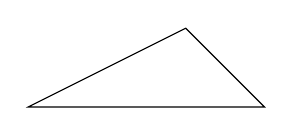
\begin{tikzpicture}
        \draw (0,0) --(2,1) --(3,0) --cycle;
    \end{tikzpicture}
\end{lstlisting}
\[
    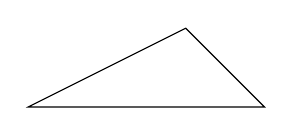
\begin{tikzpicture}
        \draw (0,0) --(2,1) --(3,0) --cycle;
    \end{tikzpicture}
\]

However, \verb|cycle| also means ``closing'', which has a better behavior than close with (0,0). Especially with thick line.
\begin{lstlisting}[
    language={[LaTeX] TeX},
    firstnumber=1,breaklines=true,gobble=4]
    
\begin{tikzpicture}
        \draw[line width=0.2cm] (0,0) --(2,1) --(3,0) --cycle;
        \draw[line width=0.2cm,xshift=4cm] (0,0) --(2,1) --(3,0) --(0,0);
    \end{tikzpicture}
\end{lstlisting}
\[
    
\begin{tikzpicture}
        \draw[line width=0.2cm] (0,0) --(2,1) --(3,0) --cycle;
        \draw[line width=0.2cm,xshift=4cm] (0,0) --(2,1) --(3,0) --(0,0);
    \end{tikzpicture}
\]

\section{Write text at a specified position using \texttt{node}}

\verb|node| operation put text on a specified position. Note that the center of the text is put to the specified position, so it is NOT annotating path. The syntax is \verb|(a,b) node{the_text};| which put the center of \verb|the_text| at (a,b). As in below list, I draw \verb|-|| to emphasize that \verb|the_text|'s center is put on the specified position.
\begin{lstlisting}[
    language={[LaTeX] TeX},
    firstnumber=1,breaklines=true,gobble=4]
    \begin{tikzpicture}
        \draw (0,0) node{数学} --(2,1) node{物理};
        \draw (0,0) -|(2,1);
    \end{tikzpicture}
\end{lstlisting}
\[
    \begin{tikzpicture}
        \draw (0,0) node{数学} --(2,1) node{物理};
        \draw (0,0) -|(2,1);
    \end{tikzpicture}
\]

\verb|node| can have shapes. The \verb|[shape=coordinate]| is actually the operation \verb|coordinate| mentioned in Section~\ref{sec:coordinate}.
\begin{lstlisting}[
    language={[LaTeX] TeX},
    firstnumber=1,breaklines=true,gobble=4]
    \begin{tikzpicture}
        \path (0,0) node[draw]{黒線} (2,0) node[fill=red!20,rotate=30]{赤背景} (4,0) node[draw,shape=circle]{丸い};
    \end{tikzpicture}
\end{lstlisting}
\[
    \begin{tikzpicture}
        \path (0,0) node[draw]{黒線} (2,0) node[fill=red!20,rotate=30]{赤背景} (4,0) node[draw,shape=circle]{丸い};
    \end{tikzpicture}
\]

Use the option \verb|at| to use \verb|node| for annotating a straight line, for example. If \verb|at| is provided, then the current position has lower priority than \verb|at|.
\begin{lstlisting}[
    language={[LaTeX] TeX},
    firstnumber=1,breaklines=true,gobble=4]
    \begin{tikzpicture}
        \draw (0,0) node at (1,1) {数学} --(2,1);
        \draw[xshift=4cm] (0,0) node[at={(1,1)},rotate=30]{物理} --({sqrt(3)},1);
    \end{tikzpicture}
\end{lstlisting}
\[
    \begin{tikzpicture}
        \draw (0,0) node at (1,1) {数学} --(2,1);
        \draw[xshift=4cm] (0,0) node[at={(1,1)},rotate=30]{物理} --({sqrt(3)},1);
    \end{tikzpicture}
\]

\verb|pos| option place the text according to the ratio set by \verb|pos|. Below 2 commands are identical, but the latter is more natural.
\begin{lstlisting}[
    language={[LaTeX] TeX},
    firstnumber=1,breaklines=true,gobble=4]
    \begin{tikzpicture}
        \draw (0,0) --(3,1)
        node[pos=0]{A} node[pos=0.3]{B}
        node[pos=0.6]{C} node[pos=0.9]{D};
        \draw[xshift=5cm] (0,0) --node[pos=0]{A} node[pos=0.3]{B} node[pos=0.6]{C} node[pos=0.9]{D} (3,1);
    \end{tikzpicture}
\end{lstlisting}
\[
    \begin{tikzpicture}
        \draw (0,0) --(3,1)
        node[pos=0]{A} node[pos=0.3]{B}
        node[pos=0.6]{C} node[pos=0.9]{D};
        \draw[xshift=5cm] (0,0) --node[pos=0]{A} node[pos=0.3]{B} node[pos=0.6]{C} node[pos=0.9]{D} (3,1);
    \end{tikzpicture}
\]

We can assign name to \verb|node| with syntax
\begin{verbatim}
    \node[name=math] at (1,2) {数学};
    \node (math) at (1,2) {数学};
\end{verbatim}
To refer to the assigned name, use \verb|(node cs:name=名前)| (when need to specify other options) or just \verb|(名前)|.

As seen below, by noticing the ``\verb|-||'', the straight line is `somewhat aligned' to the \verb|node|, instead of the specified coordinate. The \verb|node|'s coordinate is prioritized over the straight line start and end point.
\begin{lstlisting}[
    language={[LaTeX] TeX},
    firstnumber=1,breaklines=true,gobble=4]
    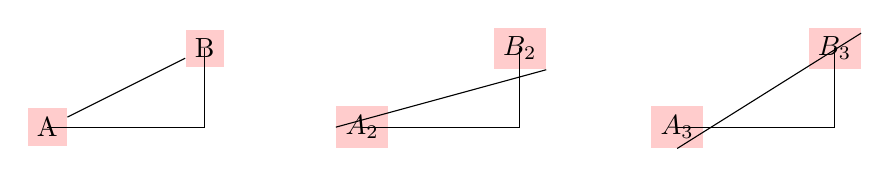
\begin{tikzpicture}
    \node[fill=red!20] (hoge) at (0,0) {A};
    \node[fill=red!20] (fuga) at (2,1) {B};
    \draw (hoge) --(fuga);
    \draw (0,0) -|(2,1);
    \node[fill=red!20] (hoge2) at (0+4,0) {$A_2$};
    \node[fill=red!20] (fuga2) at (2+4,1) {$B_2$};
    \draw (hoge2.west) --(node cs:name=fuga2,anchor=south east);
    \draw (0+4,0) -|(2+4,1);
    \node[fill=red!20] (hoge3) at (0+8,0) {$A_3$};
    \node[fill=red!20] (fuga3) at (2+8,1) {$B_3$};
    \draw (hoge3.-90) --(node cs:name=fuga3,angle=30);
    \draw (0+8,0) -|(2+8,1);
    \end{tikzpicture}
\end{lstlisting}
\[
    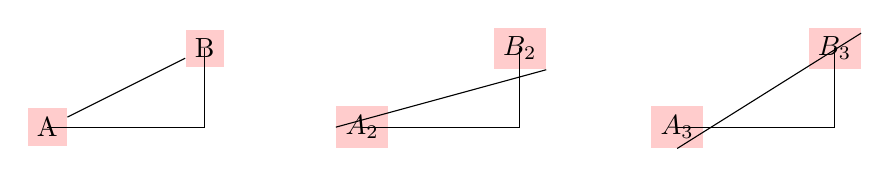
\begin{tikzpicture}
    \node[fill=red!20] (hoge) at (0,0) {A};
    \node[fill=red!20] (fuga) at (2,1) {B};
    \draw (hoge) --(fuga);
    \draw (0,0) -|(2,1);
    \node[fill=red!20] (hoge2) at (0+4,0) {$A_2$};
    \node[fill=red!20] (fuga2) at (2+4,1) {$B_2$};
    \draw (hoge2.west) --(node cs:name=fuga2,anchor=south east);
    \draw (0+4,0) -|(2+4,1);
    \node[fill=red!20] (hoge3) at (0+8,0) {$A_3$};
    \node[fill=red!20] (fuga3) at (2+8,1) {$B_3$};
    \draw (hoge3.-90) --(node cs:name=fuga3,angle=30);
    \draw (0+8,0) -|(2+8,1);
    \end{tikzpicture}
\]

Also, we can assign \verb|node|'s name in the middle of the command as below. The node \verb|x| by default is in relative position 0.5 between \verb|a| and \verb|b|.
\begin{lstlisting}[
    language={[LaTeX] TeX},
    firstnumber=1,breaklines=true,gobble=4]
    \begin{tikzpicture}
        \node (a) at (0,0) {A};
        \node (b) at (2,1) {B};
        \node (c) at (0,2) {C};
        \draw (a) -- node (x) {X} (b);
        \draw (x) --(c);
    \end{tikzpicture}
\end{lstlisting}
\[
    \begin{tikzpicture}
        \node (a) at (0,0) {A};
        \node (b) at (2,1) {B};
        \node (c) at (0,2) {C};
        \draw (a) -- node (x) {X} (b);
        \draw (x) --(c);
    \end{tikzpicture}
\]

\verb|node| without drawing the text is defined using \verb|coordinate| (only defining the coordinate's name). As in \verb|node|, \verb|coordinate| can also be defined at the middle of the command (see below coordinate \verb|(X)| and \verb|(Y)|). Please notice that \verb|node|s \verb|{A}, {B}, {C}| are drawn but they have NO names, while \verb|coordinate|s \verb|(X), (Y)| are NOT drawn but they have names.
\begin{lstlisting}[
    language={[LaTeX] TeX},
    firstnumber=1,breaklines=true,gobble=4]
    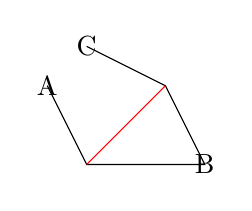
\begin{tikzpicture}
        \draw (0,1) node{A} --(0.5,0) coordinate (X)
            --(2,0) node{B} --(1.5,1) coordinate (Y)
            --(0.5,1.5) node{C};
        \draw[red] (X) --(Y);
    \end{tikzpicture}
\end{lstlisting}
\[
    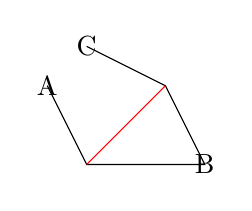
\begin{tikzpicture}
        \draw (0,1) node{A} --(0.5,0) coordinate (X)
            --(2,0) node{B} --(1.5,1) coordinate (Y)
            --(0.5,1.5) node{C};
        \draw[red] (X) --(Y);
    \end{tikzpicture}
\]

Use \verb|auto, sloped| option to name a straight line. The path direction is considered when specifying \verb|auto|.
\begin{lstlisting}[
    language={[LaTeX] TeX},
    firstnumber=1,breaklines=true,gobble=4]
    \begin{tikzpicture}
    \coordinate[label=left:B] (B) at (0,0);
    \coordinate[label={[label distance=-3pt] 20:C}] (C) at (2,1);
    \draw (B) -- node[auto,sloped]{$l_a$} (C);
    \draw (0,0) -|(2,1);
    \draw[xshift=3cm] (0,0) -- node[auto=right,sloped]{$l_b$} (2,1);
    \draw[xshift=3cm] (0,0) -|(2,1);
    \draw[xshift=6cm] (0,1) -- node[auto,sloped]{$l_c$} (2,0);
    \draw[xshift=6cm] (0,1) |-(2,0);
    \draw[xshift=9cm] (2,0) -- node[auto=right,sloped,allow upside down]{$l_d$} (0,1);
    \draw[xshift=9cm] (2,0) -|(0,1);
    \end{tikzpicture}
\end{lstlisting}
\[
    \begin{tikzpicture}
    \coordinate[label=left:B] (B) at (0,0);
    \coordinate[label={[label distance=-3pt] 20:C}] (C) at (2,1);
    \draw (B) -- node[auto,sloped]{$l_a$} (C);
    \draw (0,0) -|(2,1);
    \draw[xshift=3cm] (0,0) -- node[auto=right,sloped]{$l_b$} (2,1);
    \draw[xshift=3cm] (0,0) -|(2,1);
    \draw[xshift=6cm] (0,1) -- node[auto,sloped]{$l_c$} (2,0);
    \draw[xshift=6cm] (0,1) |-(2,0);
    \draw[xshift=9cm] (2,0) -- node[auto=right,sloped,allow upside down]{$l_d$} (0,1);
    \draw[xshift=9cm] (2,0) -|(0,1);
    \end{tikzpicture}
\]

\section{How to Use Option}

Option written right after environment, will be valid inside that environment. The \verb|[auto,x=24mm,y=12mm,->]| means, put the node's text automatically (so that the node is NOT positioned in-the-path), 1 means \qty{24}{\mm} in x-axis, 1 means in y-axis \qty{12}{\mm}, and draw arrow.
\\[1em]
\begin{minipage}{0.58 \textwidth}
    \begin{lstlisting}[
    language={[LaTeX] TeX},
    firstnumber=1,breaklines=true,gobble=8]
        \begin{tikzpicture}[auto,x=24mm,y=12mm,->]
        \node (a) at (0,1) {$a$}; \node (x) at (1,1) {$x$};
        \node (b) at (0,0) {$b$}; \node (y) at (1,0) {$y$};
        \draw (a) -- node {$\scriptstyle f$} (x);
        \draw (x) -- node {$\scriptstyle p$} (y);
        \draw (a) -- node[swap] {$\scriptstyle i$} (b);
        \draw (b) -- node[swap] {$\scriptstyle g$} (y);
        \end{tikzpicture}
    \end{lstlisting}
\end{minipage}
\hfill
\begin{minipage}{0.38 \textwidth}
    \[
        \begin{tikzpicture}[auto,x=24mm,y=12mm,->]
        \node (a) at (0,1) {$a$}; \node (x) at (1,1) {$x$};
        \node (b) at (0,0) {$b$}; \node (y) at (1,0) {$y$};
        \draw (a) -- node {$\scriptstyle f$} (x);
        \draw (x) -- node {$\scriptstyle p$} (y);
        \draw (a) -- node[swap] {$\scriptstyle i$} (b);
        \draw (b) -- node[swap] {$\scriptstyle g$} (y);
        \end{tikzpicture}
    \]
\end{minipage}
\\[1em]

\subsection{Set \texttt{.style} in Option to Use the Same Style Inside Environment}

The syntax is \verb|[スタイル名/.style=設定内容]|. This style is valid in the environment only. So, both of following commands means the same:
\\[1em]
\begin{minipage}{0.48 \textwidth}
    \begin{lstlisting}[
    language={[LaTeX] TeX},
    firstnumber=1,breaklines=true,gobble=8,numbers=none]
        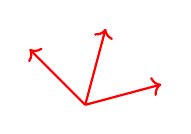
\begin{tikzpicture}
            \draw[->,color=red,thick] (0,0) --(15:1);
            \draw[->,color=red,thick] (0,0) --(75:1);
            \draw[->,color=red,thick] (0,0) --(135:1);
        \end{tikzpicture}
    \end{lstlisting}
\end{minipage}
\hfill
\begin{minipage}{0.48 \textwidth}
    \begin{lstlisting}[
    language={[LaTeX] TeX},
    firstnumber=1,breaklines=true,gobble=8,numbers=none]
        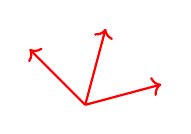
\begin{tikzpicture}[red arrow/.style={->,color=red,thick}]
            \draw[red arrow] (0,0) --(15:1);
            \draw[red arrow] (0,0) --(75:1);
            \draw[red arrow] (0,0) --(135:1);
        \end{tikzpicture}
    \end{lstlisting}
\end{minipage}

If you want to used the style at different \verb|tikzpicture| environment, then in the preamble add this:
\begin{verbatim}
    \tikzset{red arrow/.style={->,color=red,thick}}
\end{verbatim}

The \verb|.style| can receive argument.
\\[1em]
\begin{minipage}{0.78 \textwidth}
    \begin{lstlisting}[
    language={[LaTeX] TeX},
    firstnumber=1,breaklines=true,gobble=8]
        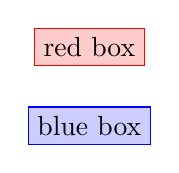
\begin{tikzpicture}[outline/.style={draw=#1,fill=#1!20},outline/.default=red]
            \node[outline] at (0,1) {red box};
            \node[outline=blue] at (0,0) {blue box};
        \end{tikzpicture}
    \end{lstlisting}
\end{minipage}
\hfill
\begin{minipage}{0.18 \textwidth}
    \[
        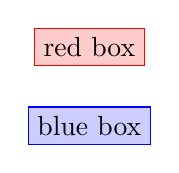
\begin{tikzpicture}[outline/.style={draw=#1,fill=#1!20},outline/.default=red]
            \node[outline] at (0,1) {red box};
            \node[outline=blue] at (0,0) {blue box};
        \end{tikzpicture}
    \]
\end{minipage}
\\[1em]

\subsection{Use \texttt{scope} to Limit the Scope of Style}

Using \verb|scope|, we can limit the scope of the style.
\\[1em]
\begin{minipage}{0.78 \textwidth}
    \begin{lstlisting}[
    language={[LaTeX] TeX},
    firstnumber=1,breaklines=true,gobble=8]
        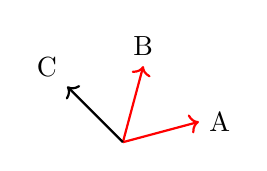
\begin{tikzpicture}[->,thick]
            \begin{scope}[draw=red]
                \draw (0,0) --( 15:1) node[right]{A};
                \draw (0,0) --( 75:1) node[above]{B};
            \end{scope}
            \draw (0,0) --(135:1) node[above left]{C};
        \end{tikzpicture}
    \end{lstlisting}
\end{minipage}
\hfill
\begin{minipage}{0.18 \textwidth}
    \[
        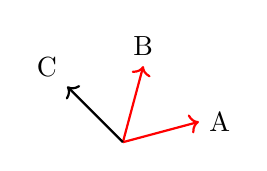
\begin{tikzpicture}[->,thick]
            \begin{scope}[draw=red]
                \draw (0,0) --( 15:1) node[right]{A};
                \draw (0,0) --( 75:1) node[above]{B};
            \end{scope}
            \draw (0,0) --(135:1) node[above left]{C};
        \end{tikzpicture}
    \]
\end{minipage}
\\[1em]

\verb|[name prefix=名前]| option can be used to make a new variable.
\\[1em]
\begin{minipage}{0.78 \textwidth}
    \begin{lstlisting}[
    language={[LaTeX] TeX},
    firstnumber=1,breaklines=true,gobble=8]
        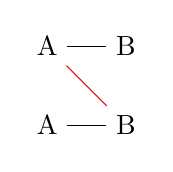
\begin{tikzpicture}
            \begin{scope}[name prefix=top-]
                \node (A) at (0,1) {A};
                \node (B) at (1,1) {B};
                \draw (A) --(B);
            \end{scope}
            \begin{scope}[name prefix=bottom-]
                \node (A) at (0,0) {A};
                \node (B) at (1,0) {B};
                \draw (A) --(B);
            \end{scope}
            \draw[red] (top-A) --(bottom-B);
        \end{tikzpicture}
    \end{lstlisting}
\end{minipage}
\hfill
\begin{minipage}{0.18 \textwidth}
    \[
        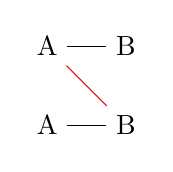
\begin{tikzpicture}
            \begin{scope}[name prefix=top-]
                \node (A) at (0,1) {A};
                \node (B) at (1,1) {B};
                \draw (A) --(B);
            \end{scope}
            \begin{scope}[name prefix=bottom-]
                \node (A) at (0,0) {A};
                \node (B) at (1,0) {B};
                \draw (A) --(B);
            \end{scope}
            \draw[red] (top-A) --(bottom-B);
        \end{tikzpicture}
    \]
\end{minipage}
\\[1em]

\subsection{\texttt{every}}

\verb|every| option will apply the option to every path, node etc. Please note the \verb|scope| will overwrite the \verb|.style|. Use \verb|.append style| to append the style (instead of just overwriting).
\\[1em]
\begin{minipage}{0.78 \textwidth}
    \begin{lstlisting}[
    language={[LaTeX] TeX},
    firstnumber=1,breaklines=true,gobble=8]
        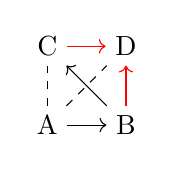
\begin{tikzpicture}[every path/.style=->]
            \node (A) at (0,0) {A};
            \node (B) at (1,0) {B};
            \node (C) at (0,1) {C};
            \node (D) at (1,1) {D};
            \draw (A) --(B);
            \begin{scope}[every path/.style=dashed]
                \draw (A) --(C);
                \draw (A) --(D);
            \end{scope}
            \begin{scope}[every path/.append style=red]
                \draw (B) --(D);
                \draw (C) --(D);
            \end{scope}
            \draw (B) --(C);
        \end{tikzpicture}
    \end{lstlisting}
\end{minipage}
\hfill
\begin{minipage}{0.18 \textwidth}
    \[
        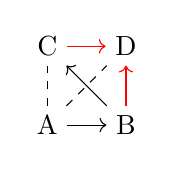
\begin{tikzpicture}[every path/.style=->]
            \node (A) at (0,0) {A};
            \node (B) at (1,0) {B};
            \node (C) at (0,1) {C};
            \node (D) at (1,1) {D};
            \draw (A) --(B);
            \begin{scope}[every path/.style=dashed]
                \draw (A) --(C);
                \draw (A) --(D);
            \end{scope}
            \begin{scope}[every path/.append style=red]
                \draw (B) --(D);
                \draw (C) --(D);
            \end{scope}
            \draw (B) --(C);
        \end{tikzpicture}
    \]
\end{minipage}
\\[1em]

\section{How to Define Coordinate and Line}
\label{sec:coordinate}

Use \verb|\coordinate| to define coordinate, along with its label and position. Use the option \verb|save path| in \verb|\path| command to define a path/line to be drawn later.
\begin{lstlisting}[
    language={[LaTeX] TeX},
    firstnumber=1,breaklines=true,gobble=4]
    \begin{tikzpicture}[every label/.style={color=blue}]
        \coordinate[label=left:Point A] (A) at (1,2);
        \coordinate[label=right:Point B] (B) at (7,4);
        \coordinate[label={[label distance=1cm,green] 60:Point C}] (C) at (2,6); % angle 60°, distance 1cm
        \path[save path=\lc,name path=lc] (A) --(B);
        \path[save path=\lb,name path=lb] (C) --(A);
        \draw[red,use path=\lc];
        \draw[cyan,use path=\lb];
        \draw (1,2) -|(7,4);
    \end{tikzpicture}
\end{lstlisting}
\[
    \begin{tikzpicture}[every label/.style={color=blue}]
        \coordinate[label=left:Point A] (A) at (1,2);
        \coordinate[label=right:Point B] (B) at (7,4);
        \coordinate[label={[label distance=1cm,green] 60:Point C}] (C) at (2,6); % angle 60°, distance 1cm
        \path[save path=\lc,name path=lc] (A) --(B);
        \path[save path=\lb,name path=lb] (C) --(A);
        \draw[red,use path=\lc];
        \draw[cyan,use path=\lb];
        \draw (1,2) -|(7,4);
    \end{tikzpicture}
\]

\section{How to Plot POINT}

To plot point explicitly, define the point style (right after \verb|\begin{tikzpicture}|), then pass it as option to \verb|node|. However, leave the \verb|node|'s text to empty (\verb|{}|). Below, the circle is on top of the node:
\begin{lstlisting}[
    language={[LaTeX] TeX},
    firstnumber=1,breaklines=true,gobble=4]
    \begin{tikzpicture}[point/.style={fill,shape=circle,inner sep=1pt,outer sep=0pt}]
        \node[point] (c) at (0,0) {};
        \node[point] (x) at (0.7,0.3) {};
        \draw[red,thick] (c) --(x);
        \node[draw=green,very thick,circle through=(x)] at (c) {};
    \end{tikzpicture}
\end{lstlisting}
\[
    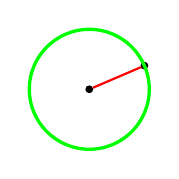
\begin{tikzpicture}[point/.style={fill,shape=circle,inner sep=1pt,outer sep=0pt}]
        \node[point] (c) at (0,0) {};
        \node[point] (x) at (0.7,0.3) {};
        \draw[red,thick] (c) --(x);
        \node[draw=green,very thick,circle through=(x)] at (c) {};
    \end{tikzpicture}
\]

To make the point on top of the circle, first just define \verb|coordinate|, then at the end use \verb|\node[point]| to draw the point defined by the \verb|coordinate|.
\begin{lstlisting}[
    language={[LaTeX] TeX},
    firstnumber=1,breaklines=true,gobble=4]
    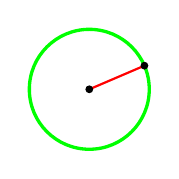
\begin{tikzpicture}[point/.style={fill,shape=circle,inner sep=1pt,outer sep=0pt}]
        \coordinate (c) at (0,0);
        \coordinate (x) at (0.7,0.3);
        \draw[red,thick] (c) --(x);
        \node[draw=green,very thick, circle through=(x)] at (c) {};
        \node[point] at (c) {};
        \node[point] at (x) {};
    \end{tikzpicture}
\end{lstlisting}
\[
    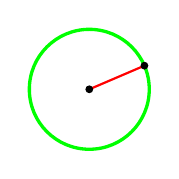
\begin{tikzpicture}[point/.style={fill,shape=circle,inner sep=1pt,outer sep=0pt}]
        \coordinate (c) at (0,0);
        \coordinate (x) at (0.7,0.3);
        \draw[red,thick] (c) --(x);
        \node[draw=green,very thick, circle through=(x)] at (c) {};
        \node[point] at (c) {};
        \node[point] at (x) {};
    \end{tikzpicture}
\]

\cprotect \section{Difference between \verb|\draw|, \verb|\fill|, \verb|\shadedraw|, and \verb|\shade|} % chktex 1

\verb|\draw|, \verb|\shadedraw| will draw the shape, while \verb|fill|, \verb|shade| will draw the inner region only.
\begin{lstlisting}[
    language={[LaTeX] TeX},
    firstnumber=1,breaklines=true,gobble=4]
    
\begin{tikzpicture}
        \draw[blue] (0,0) rectangle+(1,1);
        \draw[blue,fill=red] (0,-1.5) rectangle+(1,1);
        \fill[red] (0,-3.0) rectangle+(1,1);
        \shadedraw[blue,top color=green,bottom color=orange] (0,-4.5) rectangle+(1,1);
        \shade[top color=cyan,bottom color=yellow] (0,-6.0) rectangle+(1,1);
    \end{tikzpicture}
\end{lstlisting}
\[
    
\begin{tikzpicture}
        \draw[blue] (0,0) rectangle+(1,1);
        \draw[blue,fill=red] (0,-1.5) rectangle+(1,1);
        \fill[red] (0,-3.0) rectangle+(1,1);
        \shadedraw[blue,top color=green,bottom color=orange] (0,-4.5) rectangle+(1,1);
        \shade[top color=cyan,bottom color=yellow] (0,-6.0) rectangle+(1,1);
    \end{tikzpicture}
\]

\section{How to Draw Angle Bisector Line in Triangle}

Refer to \url{https://tex.stackexchange.com/questions/233246/create-angle-bisectors-in-tikz} on how to write angle bisector without using \verb|tikz-euclid|. However, if you pressed \verb|Command+Option+J| then the region of belows diagram are very big. This is due to using helper-coordinate inside \verb|\bissectrice|. Use \verb|\clip| to crop in only elements which are shown in the diagram. Or, \verb|\useasboundingbox| is maybe better because it does not forcely clipped the region outside the bounding box, and good to adjust white space area. Both must be used at the top, right after \verb|\begin{tikzpicture}|.
\begin{lstlisting}[
    language={[LaTeX] TeX},
    firstnumber=1,breaklines=true,gobble=4]
    \begin{tikzpicture}
    % \clip (-1,-0.5) rectangle (7,4.5);
    \useasboundingbox (-1,-0.5) rectangle (7,4.5);
    \coordinate[label=left:A] (A) at (0,0);
    \coordinate[label=right:B] (B) at (6,2);
    \coordinate[label={[label distance=0.1cm] above:C}] (C) at (1,4);
    \path[save path=\lc,name path=lc] (A) --(B);
    \path[save path=\lb,name path=lb] (C) --(A);
    \path[save path=\la,name path=lb] (B) --(C);
    \draw[dashed,use path=\lc];
    \draw[dashed,use path=\lb];
    \draw[use path=\la];
    \bissectrice{C}{A}{B}{R}
    \bissectrice{A}{B}{C}{S}
    \draw[red] (A) --(R);
    \path[name intersections={of=BisCAB and BisABC, by=O}];
    \node[draw=blue] at (O) [circle through={($(C)!(O)!(B)$)}] {};
    \end{tikzpicture}
\end{lstlisting}
\[
    \begin{tikzpicture}
    % \clip (-1,-0.5) rectangle (7,4.5);
    \useasboundingbox (-1,-0.5) rectangle (7,4.5);
    \coordinate[label=left:A] (A) at (0,0);
    \coordinate[label=right:B] (B) at (6,2);
    \coordinate[label={[label distance=0.1cm] above:C}] (C) at (1,4);
    \path[save path=\lc,name path=lc] (A) --(B);
    \path[save path=\lb,name path=lb] (C) --(A);
    \path[save path=\la,name path=lb] (B) --(C);
    \draw[dashed,use path=\lc];
    \draw[dashed,use path=\lb];
    \draw[use path=\la];
    \bissectrice{C}{A}{B}{R}
    \bissectrice{A}{B}{C}{S}
    \draw[red] (A) --(R);
    \path[name intersections={of=BisCAB and BisABC, by=O}];
    \node[draw=blue] at (O) [circle through={($(C)!(O)!(B)$)}] {};
    \end{tikzpicture}
\]

Below is the example shown in the \texttt{stackexchange.com}, modified a little bit.
\begin{lstlisting}[
    language={[LaTeX] TeX},
    firstnumber=1,breaklines=true,gobble=4]
    \begin{tikzpicture}
    % \clip (-3,-1) rectangle (9,7.5);
    \useasboundingbox (-3,-1) rectangle (9,7.5);
    \coordinate[label=below left:$C$](C) at (-2,0);
    \coordinate[label=below right:$A$](A) at (8,0);
    \coordinate[label=above left:$B$] (B) at (0,7);
    \coordinate[label=above right:$D$](D) at ($(A)!(C)!(B)$);
    \draw (A) -- (B) -- (C) -- cycle;
    \draw (C) -- (D);

    \bissectrice[draw,blue]{B}{C}{D}{R}[1.1][1.2]
    \bissectrice[draw,dashed]{D}{B}{C}{S}
    \bissectrice[draw,dashed]{C}{D}{B}{T}

    \path[name intersections={of=BisBCD and BisDBC, by=O}] ;

    \node[draw=red] at (O) [circle through={($(C)!(O)!(B)$)}] {};
    \end{tikzpicture}
\end{lstlisting}
\[
    \begin{tikzpicture}
    % \clip (-3,-1) rectangle (9,7.5);
    \useasboundingbox (-3,-1) rectangle (9,7.5);
    \coordinate[label=below left:$C$](C) at (-2,0);
    \coordinate[label=below right:$A$](A) at (8,0);
    \coordinate[label=above left:$B$] (B) at (0,7);
    \coordinate[label=above right:$D$](D) at ($(A)!(C)!(B)$);
    \draw (A) -- (B) -- (C) -- cycle;
    \draw (C) -- (D);

    \bissectrice[draw,blue]{B}{C}{D}{R}[1.1][1.2]
    \bissectrice[draw,dashed]{D}{B}{C}{S}
    \bissectrice[draw,dashed]{C}{D}{B}{T}

    \path[name intersections={of=BisBCD and BisDBC, by=O}] ;

    \node[draw=red] at (O) [circle through={($(C)!(O)!(B)$)}] {};
    \end{tikzpicture}
\]

\section{Draw Axis, Grid, Tick}

\begin{lstlisting}[
    language={[LaTeX] TeX},
    firstnumber=1,breaklines=true,gobble=4]
    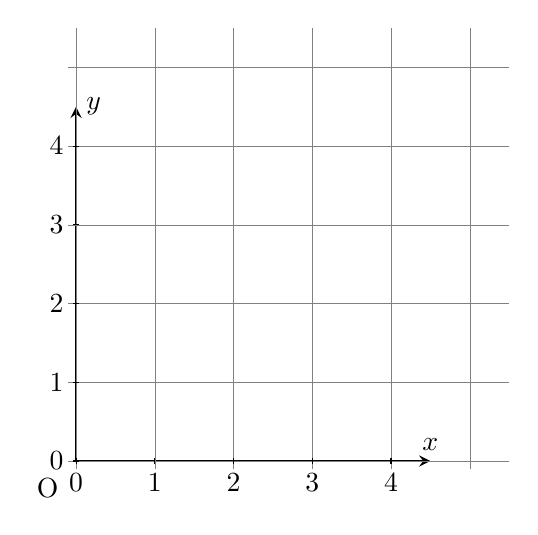
\begin{tikzpicture}
    \draw[->,>=stealth,thick] (0,0) --(4.5,0) node[above]{$x$}; %x軸
    \draw[->,>=stealth,thick] (0,0) --(0,4.5) node[right]{$y$};
    \draw (-0.1,-0.1) node[below left]{O}; %原点
    \draw[step=1cm,help lines] (-0.1,-0.1) grid(5.5,5.5);
    \foreach \x in {0,1,2,3,4}
    \draw (\x cm,1pt) -- (\x cm,-1pt) node[anchor=north] {$\x$};
    \foreach \y in {0,1,2,3,4}
    \draw (1pt,\y cm) -- (-1pt,\y cm) node[anchor=east] {$\y$};
    \end{tikzpicture}
\end{lstlisting}
\[
    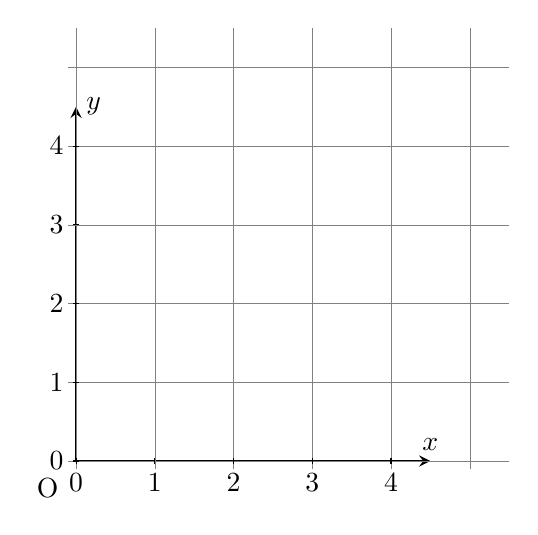
\begin{tikzpicture}
    \draw[->,>=stealth,thick] (0,0) --(4.5,0) node[above]{$x$}; %x軸
    \draw[->,>=stealth,thick] (0,0) --(0,4.5) node[right]{$y$};
    \draw (-0.1,-0.1) node[below left]{O}; %原点
    \draw[step=1cm,help lines] (-0.1,-0.1) grid(5.5,5.5);
    \foreach \x in {0,1,2,3,4}
    \draw (\x cm,1pt) -- (\x cm,-1pt) node[anchor=north] {$\x$};
    \foreach \y in {0,1,2,3,4}
    \draw (1pt,\y cm) -- (-1pt,\y cm) node[anchor=east] {$\y$};
    \end{tikzpicture}
\]

\section{How to Annotate Line with Its Length}

TODO on how to annotate line with for example its length.

\end{document}
